\section{Nuclear Fission and Neutron Spectra}

Radiation damage in a reactor is caused by several projectiles.  Fission fragments are heavy, contain charged particles and lose energy close to their source.  Gamma rays ionise may excite atoms and electrons, but do not have the momentum to knock atoms out of place.  Fast neutrons, however, may impart a great deal of momentum to a target atom and, as they are neutral, travel much further into a material than fission fragments.

One fuel source for many of the Gen III+ and Gen IV reactors is Uranium-235, whether as enriched Uranium or otherwise.  The neutron/s released by the fission of Uranium-235 atoms have a spectra of energy which may roughly be split into four categories: cold (below 0.025eV), thermal (0.025eV), slow and intermediate (above 0.025eV and below 1MeV) and fast (1MeV and above).

Thermal and slow/intermediate neutrons cause damage in their own particular way, as they are captured by and transmute the atoms within the target material.  Fast neutrons 


\begin{figure}[tbp]
  \begin{center}
    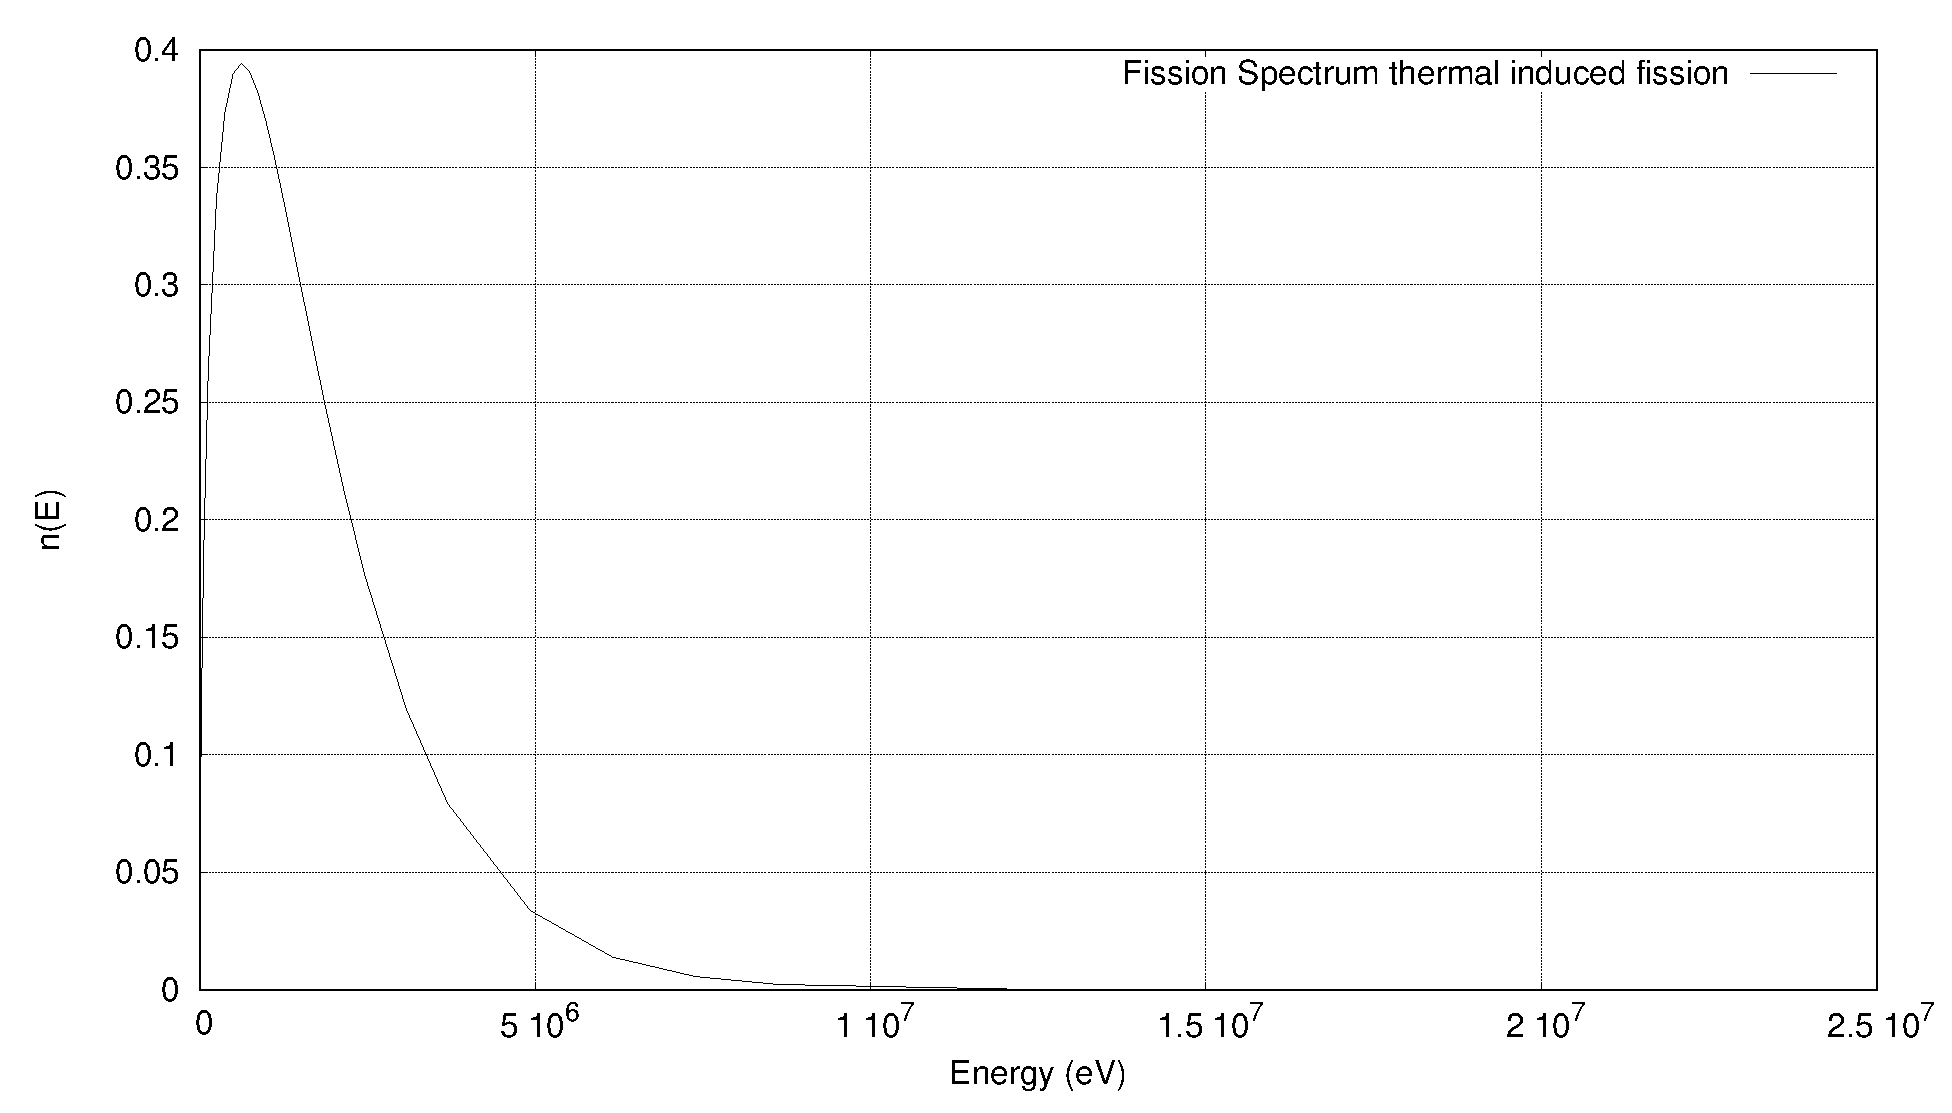
\includegraphics[width=15.0cm]{chapters/introduction/plots/fission_spectra/fission_spectra.eps}
    \captionsetup{font={it}}
    \caption{Fission Spectra}
    \label{fig:electricityusagesuk}
  \end{center}
\end{figure}





reference literature neutron damage

Neutrons 





